\section{High-Level Risks}

Risks allow us to measure the probability of not accomplishing a defined goal and its consequences for the project. Their identification is crucial in order to know in advance the factors that could make the project go wrong.

The determination of the risks is an iterative process because, when the different activities progress through the specified time, new risks or uncertainties can appear. The main structures and departments of the team have to participate in this task in order to spot as many risks as possible. Even stakeholders have to provide additional information and points of view.

The factors that are used in the identification process are: enterprise environmental factors, organizational process assets, the project scope statement and the project management plan.

After analysing these points, risks have been classified in two groups: External risks, which are the ones that our team cannot control, so they are inevitable, and Internal risks, which can be detected in advance and be addressed properly by our own members.

The main identified risks are shown below.

\textbf{External risks}

\begin{itemize}
	
	\item \textbf{Competitors appearance:} The emergence of other companies that could offer the same product. This could modify the benefits of our company.
	
	\item \textbf{Delays in external deliverables:} If the products that the company orders do not arrive at the predicted time all the processes can experience a delay, incrementing costs.
	
	\item \textbf{Economical market issues:} During the period of time that the project is executed, there could be large-scale economic crisis.
	
	\item \textbf{Exit of a member of the corporation:} For different reasons, a member that had committed to the project could leave it before than expected.
	
	\item \textbf{Components and raw materials quality:} The ordered equipment or materials could not be in good condition, delaying processes and increasing costs.
	
\end{itemize}

\textbf{Internal risks}

\begin{itemize}
	
	\item \textbf{Delays in deliverables:} The deliverables could not be completed at the time of their corresponding deadlines, leading to an increase of costs and a delay of all the schedule of the project.
	
	\item \textbf{Cost forecasts are inaccurate:} The financial predictions could be wrong or different issues may occur increasing the total cost of the project.
	
	\item \textbf{Lack of communication:} The absence of a proper communication method or channel might affect the quality of the product, the fulfilment of the deadlines or a good coordination between members and departments.
	
	\item \textbf{Lack of technology improvement:} The main goal of the project is to innovate but it could happen that the company did not find the way to improve enough the different technologies.
	
	\item \textbf{Lack of information:} Discovering new technologies implies working with leading-edge science. It could occur that the team does not have access to the last improvements or patents.
	
	\item \textbf{Low team motivation:} The team could lose motivation, which would lead the project to take more time and costs to be completed.
	
	\item \textbf{Unsuccessful quality control:} The quality of some component, product or deliverable may not be as it is expected and established in the acceptance criteria.
	
	\item \textbf{Lack of responsibilities:} The responsibilities taken by the members of the team or the stakeholders could not be accomplished as expected.
	
	\item \textbf{Conflicts between members:} There could be a disagreement over the project issues between executive members.
	
	\item \textbf{Infeasible design:} The design could turn out to be excessively costly or not possible to be built.
	
	\item \textbf{Technology components have security vulnerabilities:} Security vulnerabilities are unwanted in high-tech projects if some government is interested in using the technology.
	
	\item \textbf{Organization issues:} The project could be not well organized in terms of timing, activities, etc. and the schedule may be always changing.
	
	\item \textbf{Stakeholders desertion:} The abandonment of a stakeholder could occur for several reasons, leaving the project without its contribution.
	
	\item \textbf{Stakeholders conflict:} Different executives of the stakeholders could have a disagreement over the project at an executive level.
	
	
\end{itemize}

When managing risks, both the probability and their consequences have to be considered. During the project, each event will be classified into different types of risks. In a general level, they can be classified into low, moderate and high risks. The following figure represents the classification depending on the probability and the magnitude of impact.

\begin{figure}[H]
	\centering
	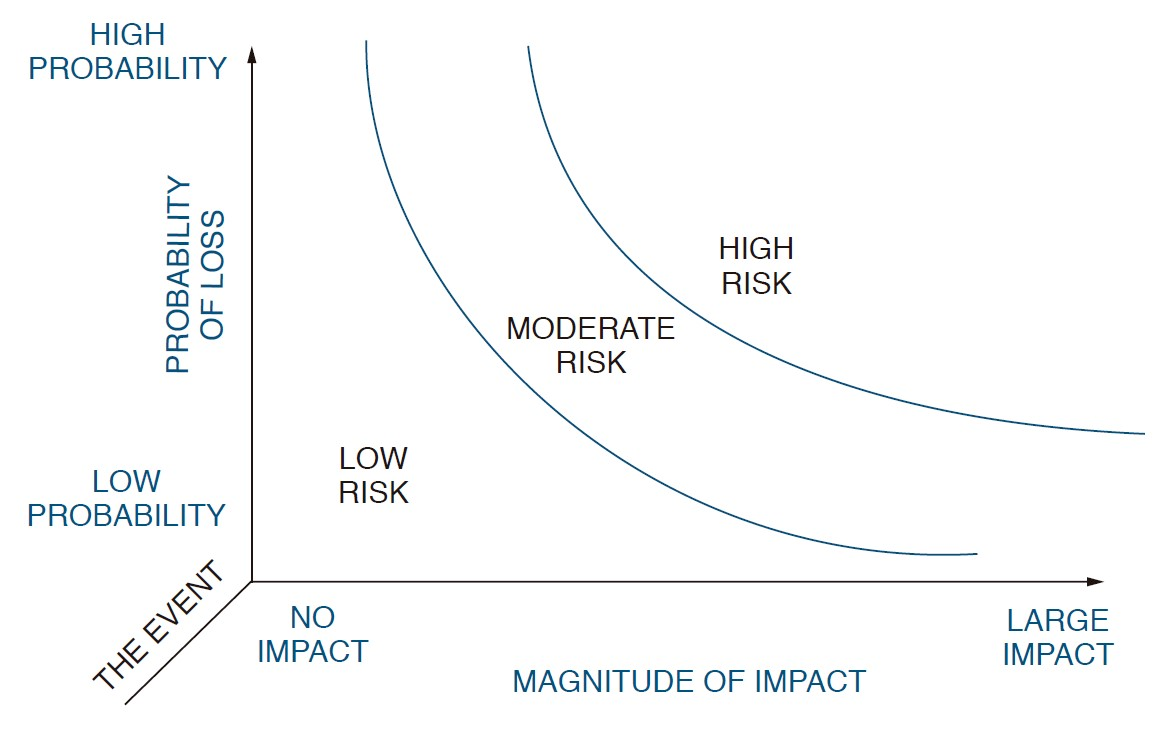
\includegraphics[width=0.65\linewidth]{./images/risks1}
	\caption{Overall risk is a function of its components \cite{Kerzner2009}.}
	\label{fig:risks1}
\end{figure}

During the following stages of the project, each risk will be assessed with the Probability and Impact Matrix. It is a tool which allows the team to rate risks on their probability and impact in the project. This gives a quick and clear view of which risk is more important to control.

\begin{figure}[H]
	\centering
	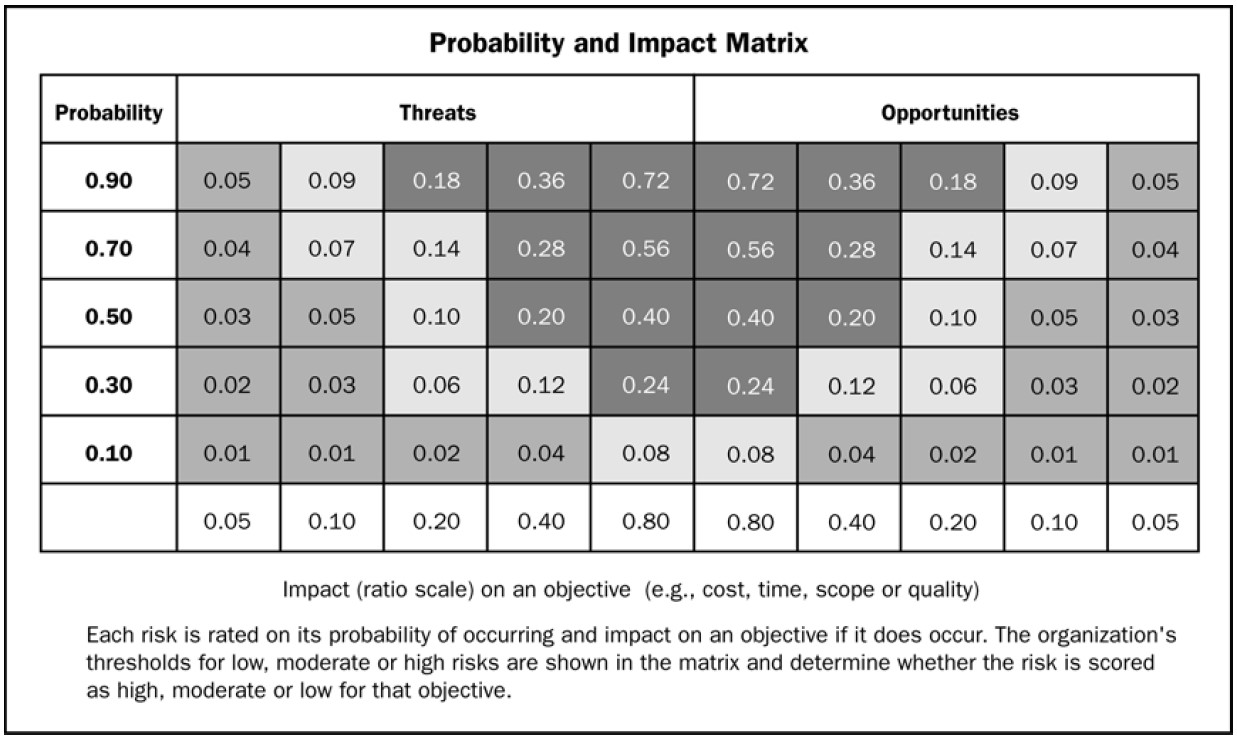
\includegraphics[width=\linewidth]{./images/risks2}
	\caption{Probability and Impact Matrix \cite{ProjectManagementInstitute2004}.}
	\label{fig:risks2}
\end{figure}
